\chapter{Технологический раздел}
\section{Выбор  языка программирования}
Выбранный язык – С++.
Причины:
\begin{enumerate}
	 \item Компилируемый язык со статической типизацией. 
	 \item Сочетание высокоуровневых и низкоуровневых средств.
	 \item Реализация ООП.
	 \item Наличие удобной стандартной библиотеки шаблоны
	 \end{enumerate}
\section{Выбор вспомогательных библиотек}
Для реализации программы была выбрана библиотека Qt.
\begin{enumerate}
	\item Широкие возможности работы с изображениями, в том числе и попиксельно
	\item Наличии более функциональных аналогов стандартной библиотеки шаблонов в том числе для разнообразных структур данных
\end{enumerate}
\subsection{Диаграмма классов}
\begin{figure}[h!]
	\centering
	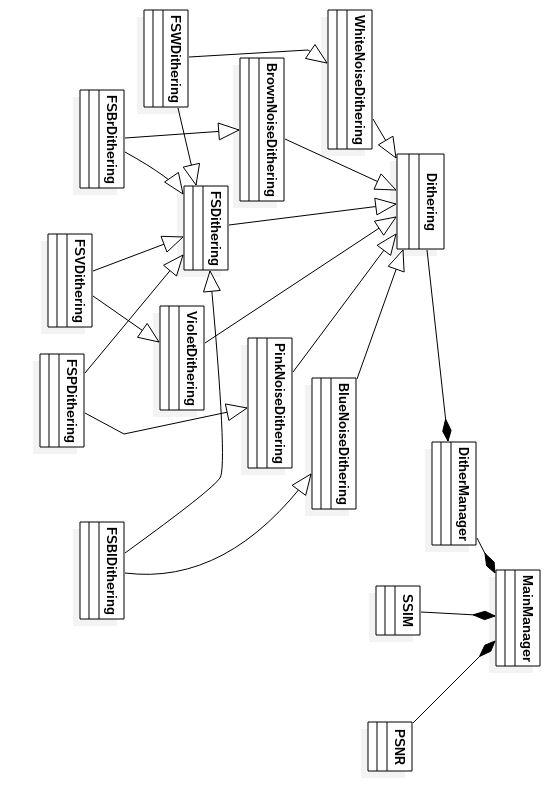
\includegraphics[width=\textwidth]{img/diagramm.png}
	\caption{Диаграмма классов}
	\label{fig:spire03}
\end{figure}

%%% Local Variables:
%%% mode: latex
%%% TeX-master: "rpz"
%%% End:
